% This is samplepaper.tex, a sample chapter demonstrating the
% LLNCS macro package for Springer Computer Science proceedings;
% Version 2.21 of 2022/01/12
%
\documentclass[runningheads]{llncs}
%\documentclass{article}

%
\usepackage[T1]{fontenc}
% T1 fonts will be used to generate the final print and online PDFs,
% so please use T1 fonts in your manuscript whenever possible.
% Other font encondings may result in incorrect characters.
%
\usepackage{graphicx}
% Used for displaying a sample figure. If possible, figure files should
% be included in EPS format.
%
% If you use the hyperref package, please uncomment the following two lines
% to display URLs in blue roman font according to Springer's eBook style:
%\usepackage{color}
%\renewcommand\UrlFont{\color{blue}\rmfamily}
%\urlstyle{rm}
%
\usepackage{listings}
\usepackage{xcolor}
\usepackage{tabularx}
\usepackage{array} % For better column alignment
\usepackage{adjustbox} % For scaling the table if needed
\usepackage{multirow} % Optional: For more advanced row manipulation
\usepackage{pgfplots}  
\usepackage{pgfplotstable}
\pgfplotsset{compat=1.18}
\renewcommand{\arraystretch}{1.5} % Adjust row height for better readability

\lstset{
    language=bash,
    basicstyle=\ttfamily\small, % Font style and size
    keywordstyle=\color{blue}, % Keywords color
    commentstyle=\color{green!60!black}, % Comments color
    stringstyle=\color{red}, % Strings color
    showstringspaces=false, % Do not show spaces in strings
    frame=single, % Adds a frame around the code
    breaklines=true, % Allow breaking of long lines
}
\begin{document}
%
\title{SAT Benchmarks from Circuits with Random Gates}
%
%\titlerunning{Abbreviated paper title}
% If the paper title is too long for the running head, you can set
% an abbreviated paper title here
%
\author{Modoac\u a Iulia \and
Todoca Ioana \and
\c Sapc\u a Miruna \and
 Bogdan Jude}
%
% First names are abbreviated in the running head.
% If there are more than two authors, 'et al.' is used.
%
\institute{West University of Timi\c soara
\\
\url{https://info.uvt.ro/} 
}
%
\maketitle              % typeset the header of the contribution
%
\begin{abstract}
Satisfiability solving, the problem of deciding
whether the variables of a propositional formula can be assigned in such a way that the formula evaluates to true, is one of the classic problems in computer science.  It is
of practical interest because modern SAT-solvers can be used to
solve many important and practical problems.

In this paper, we aim to investigate the utility of the MiniSat solver, in solving complex propositional problems. We will look at technical details regarding the implementation and operation of the MiniSat solver, including basic algorithms such as DPLL (Davis-Putnam-Logemann-Loveland) and CDCL (Conflict-Driven Clause Learning). So, the main objectives of this paper are the presentation of the MiniSat solver and its installation on two different computing environments, followed by the running of a benchmark used in the SAT 2024 competition, the highlighting and interpretation of the results obtained and the enumeration of the challenges encountered during the realization of the project.

\keywords{MiniSAT  \and SAT solver \and Propositional logic}
\end{abstract}
%
%
%
\section{Introduction}

Boolean satisfiability (SAT) has been studied for the last twenty years. Due to developments, SAT solvers can now be applied to a wide range of tasks, such as the official validation of digital designs and many more. SAT solvers' capabilities and performance are still constrained, though. Practically speaking, SAT solvers are used as blackboxes in a large number of current applications. This means that the problem is converted into a monolithic conjunctive normal form instance and then sent to the SAT solver without any communication between the application and the SAT solver. Conflict-driven SAT-solvers are SAT-solvers that use the DPLL method, backtracking with conflict analysis and clause recording (sometimes called learning), and Boolean constraint propagation (BCP) using watched literals. These solvers can be conceptually divided into three main components:

\vspace{15mm}

\begin{enumerate}
  \item Representation. The SAT instance must be internally represented using efficient data structures, along with any derived information.

  \item Inference: While brute-force search alone is rarely sufficient, solvers rely on mechanisms to compute and propagate the direct implications of the current state of information. Inference is typically combined with search to ensure completeness.
  
  \item Search.  Search can be seen as another method of deriving information. 
  
  
\end{enumerate}

A typical conflict-driven SAT solution handles assignments and clauses (of two or more literals). Despite being legally classified as unit clauses, assignments are often treated differently due to their special qualities. Unit propagation is the major inference method used by these solvers; when a phrase becomes unit under the current assignment (all literals except one are false), the remaining unbound literal is set to true. This action may cause more clauses to become units, which will spread until no more information can be determined.


Modern SAT-solvers, like MiniSat, expand upon this fundamental structure by including strategies like conflict-driven learning. In order to determine the reason of a conflict that emerges under the present assignment, the solver traces the problem back through variable assignments. Building a conflict clause—a fresh clause that stops the same conflicting assignment from happening again—is part of this process. This clause is then added to the clause database. Learned clauses serve a dual purpose: they guide backtracking and accelerate future conflict resolution by "caching" the reason for the conflict.

MiniSat uses watched literals to propagate Boolean constraints, a technique inspired by CHAFF, a method created by Princeton University researchers to solve instances of the Boolean satisfiability issue in programming using the DPLL algorithm. Using this method, a clause's two unbound literals are marked as monitored. These literals are monitored for changes.

Strategic conflict analysis is also beneficial to the learning process. Conflict clauses direct backtracking when conflicts arise in order to prevent unnecessary search paths. Non-chronological backtracking, in which the solution skips levels that are not directly related to the dispute and returns to the most fitted decision level, can improve this tracking.

While the addition of learned clauses accelerates future inferences, an excessive number of such clauses can slow down propagation. To address this, MiniSat minimizes the quantity of learnt clauses by keeping just those that meet heuristic criteria and are considered useful.

Custom Boolean constraints can be integrated into MiniSat thanks to its extensibility, which affects its search, inference, and representation techniques. Therefore, MiniSat preserves clarity while supporting a broad range of problem domains by defining the dependencies between the SAT algorithm and constraint implementation. The solver will continue to be strong and flexible for a variety of applications thanks to this design.

\subsection{MiniSAT overview}
MiniSat is a efficient and extensible Boolean Satisfiability (SAT) solver that has become very important in the SAT-solving community. SAT problems are foundational in fields like formal verification, artificial intelligence, constraint satisfaction, and optimization. MiniSat has been widely adopted in both academia and industry due to its combination of simplicity, robustness, and performance, making it suitable for research, educational purposes, and practical applications.
\\
At the heart of MiniSat is the implementation of the Conflict-Driven Clause Learning (CDCL) algorithm, a technique for SAT solving. CDCL enables the solver to learn from conflicts encountered during the search process, creating new clauses that prevent the same mistakes from being repeated. The learned clauses are generated using the First-UIP (Unique Implication Point) scheme, which ensures efficiency. To facilitate fast clause propagation, MiniSat uses a two-literal watching scheme, a mechanism that tracks only two literals per clause to reduce computational overhead during unit propagation. In order to make sure that the solver focuses on the most likely areas of the search space, activity-based heuristics such as Variable State Independent Decaying Sum (VSIDS) prioritize variable assignments according to their relevance to recent conflicts.
\\
MiniSat incorporates several strategies to enhance its efficiency. It uses restart mechanisms to periodically reset the search, allowing it to explore new areas of the solution space. Simplification techniques, such as clause subsumption and self-subsuming resolution, are applied to reduce redundancy in the clause database, improving performance. Additionally, MiniSat facilitates incremental SAT solving, which allows users to reuse previously learned sentences and variable states to answer related problems iteratively. Applications where issue instances change over time, such formal verification or optimization, benefit from this capability. 
\\
 MiniSat has also served as a foundation for developing more advanced solvers, including Glucose and CryptoMiniSat. Additionally, its influence is evident in SAT competitions, where its concepts and methodologies have shaped the development of other solvers.
\\
There are many different uses for MiniSat, such as formal verification field for tasks such as equivalency checking, software bug discovery, and hardware model checking. Because it can manage scheduling, resource allocation, and optimization issues, it is also used in constraint satisfaction situations. Its solving capability makes it a useful tool for dynamic systems.
\\

\subsection{Installing and configuring MiniSAT}

To install MiniSAT on Ubuntu through WSL on a Windows system, the first step was to ensure that the system packages were up-to-date. This was achieved by running the commands \textit{sudo apt update} and \textit{sudo apt upgrade} in the Ubuntu terminal, which refreshed the package list and installed any available updates. Next, MiniSAT was installed using the apt package manager with the command \textit{sudo apt install minisat}. After the installation process was completed, the installation was verified by running the  \textit{minisat} command in the terminal, confirming that the program was installed successfully and was ready for use. This process allowed MiniSAT to be set up and ready for solving Boolean satisfiability problems within the Ubuntu environment on WSL, running on a Windows system. 

\section{Experiments and benchmarking}
As was proven before, MiniSat is a reliable tool for conducting experiments and benchmarking in the domain of SAT solving. It is a good option for testing new concepts in algorithms and heuristics due to its simplicity and strong performance. MiniSat can be used as a baseline solver to evaluate the effectiveness of new techniques, such as alternative decision heuristics, preprocessing methods, or conflict analysis strategies. In addition, it is easy to modify and integrate experimental features due to its compact codebase.
\\
All these features have made MiniSat's efficiency a popular choice for benchmarking SAT-solving performance across a variety of problem domains. It has been used extensively in SAT competitions to evaluate the relative strengths of different solvers under standardized conditions. Its support for standard input formats, such as DIMACS for CNF, ensures compatibility with widely available benchmark suites, such as those from SAT Challenge and SAT Race. These benchmarks include problems from real-world applications, such as hardware and software verification and cryptography.
\subsection{The random-circuits benchmark}

Boolean circuits are made of logic gates and can be represented as CNF formulas.  SAT solvers are known to be more efficient in circuit-based formulas by identifying specific types of gates and processing them with special techniques.

Some researchers proposed a CNF generator that can build circuits made of gates that map a number of input bits into a number of randomly chosen output bits, which turn them into SAT problems.

The construction of the circuits is split into two main parts: the construction of a single random gate and the construction of an entire circuit. For generating a single random gate the number of input and output bits should be given. To generate an entire circuit we should consider the number of input and output bits, the number of the gates and a parameter that limits the distance between the input and output variables of a gate. Therefore, a circuit can be generated by adding gates and connecting them. All gates have the same number of input bits and output bits and every input can be only connected to multiple inputs, but one output can be connected to multiple inputs.

Up until now, we noticed how the circuits are actually created. C. Franck from Univeristy of Luxembourg aimed to turn these circuits into a satisfiable SAT problem by choosing a random assignment of the input bits, computing the resulting output bits, and then adding the assignment of these output bits the CNF formula. This led to a SAT problem that consists in finding a model that produces the right output bits.

\subsection{Experimental setup}

Since we wanted to evaluate how the running times of CNF files in MiniSAT vary depending on the hardware configuration of each machine, we used for running the random-circuits benchmark two computing environments with the following specifications:\\

Computer 1: 
\begin{itemize}
  \item CPU: Intel i7-8565U @ 1.99 GHz
  \item RAM: 16 GB
   \item Operating system: Windows 11
\end{itemize}

Computer 2: 
\begin{itemize}
  \item CPU: Intel i7-8550U @ 1.80 GHz
  \item RAM: 16 GB
   \item Operating system: Windows 10
\end{itemize}

Also, a bash script was designed to automate the processing of .sanitized.cnf files using the SAT solver called minisat. Below is presented a flow diagram that shows the functionality of this script: 
\begin{figure}[h] 
    \centering
    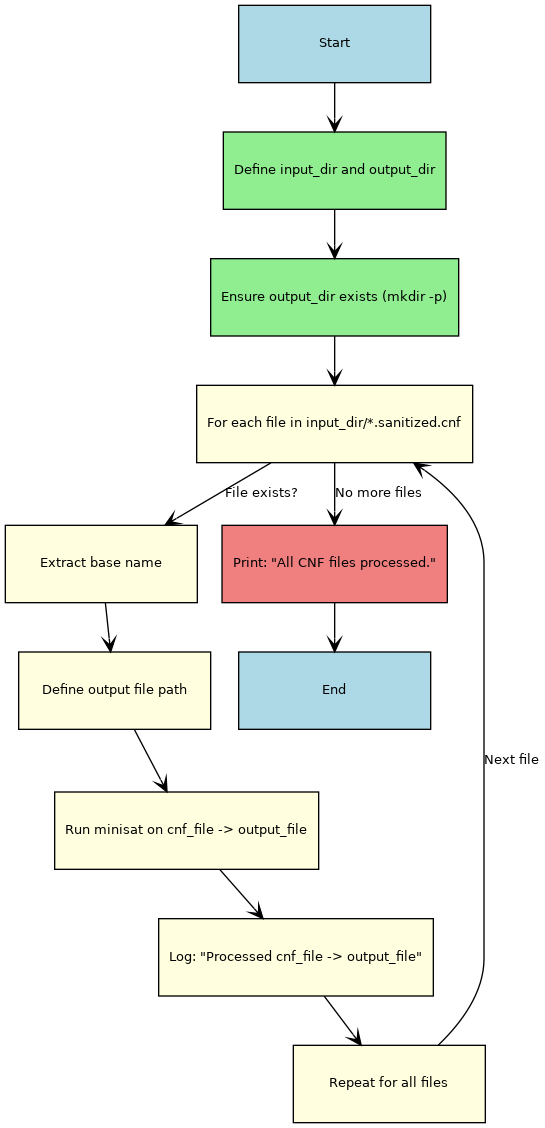
\includegraphics[height=8cm]{minisat_flow.png} 
    \label{fig:sample}
\end{figure}

The script reads .sanitized.cnf files from a designated input directory, with a for loop it iterates over all files in the input directory that have the .sanitized.cnf extension. Then it runs the minisat solver on the current file, the output of the solver is saved to the corresponding output file. After all files have been processed, a message is displayed in the terminal to confirm that the script has completed its task.
\\
\\
From the benchmark database we chose the family "random-circuits" to which it belonged 15 benchmarks. In 24 hours, with the Computer1, its specifications enumerated above, it was managed to run with minisat 8 benchmarks. \\


\begin{adjustbox}{width=\textwidth,center}
\begin{tabular}{|p{16cm}|c|c|c|}
\hline
\textbf{Benchmark Name} & \textbf{Running Time} & \textbf{File Size} & \textbf{MiniSAT Result} \\ \hline
7ac7fabd8c078aea420087a0c80e5563-circuit\_32in32out\_with\_400gates\_6in6out\_dist64\_seed1 & 77.6646 s & 98.635 kb & SAT \\ \hline
6f7a0e1cf94b6b26eafc08a827a692ce-circuit\_64in64out\_with\_64gates\_8in5out\_dist256\_seed1 & 125.385 s & 27.676 kb & SAT \\ \hline
37ca184832fc6fa43a22ae900f1756a2-circuit\_32in32out\_with\_350gates\_6in6out\_dist64\_seed1 & 67.9899 s & 85.275 kb & SAT \\ \hline
71ec94c233016219e12d671594dc88e5-circuit\_32in32out\_with\_70gates\_7in7out\_dist128\_seed1 & 1032.41 s & 68.994 kb & SAT \\ \hline
170b13af977e962321c493544b2bd0a9-circuit\_48in64out\_with\_800gates\_4in4out\_dist128\_seed4 & 1088.31 s & 8.123 kb & SAT \\ \hline
396fd56f3fd7b85afbba4254ea6e746c-circuit\_32in32out\_with\_80gates\_7in7out\_dist128\_seed1 & 512.985 s & 79.170 kb & SAT \\ \hline
8942dca5dc0876fc3f723f738d72de1c-circuit\_32in32out\_with\_64gates\_8in6out\_dist128\_seed2 & 2186.12 s & 61.300 & SAT \\ \hline
303480ca7e8322d771c94caf4ebd4e95-circuit\_48in64out\_with\_700gates\_4in4out\_dist128\_seed1 & 13.2318 s & 7.046 kb & SAT \\ \hline
\end{tabular}
\end{adjustbox}
\\


The second computer run 10 benchmarks in hours. The results and the specific running time for each benchmark can be found in the following table. \\

\begin{adjustbox}{width=\textwidth,center}
\begin{tabular}{|p{16cm}|c|c|c|}
\hline
\textbf{Benchmark Name} & \textbf{Running Time} & \textbf{File Size} & \textbf{MiniSAT Result} \\ \hline
170b13af977e962321c493544b2bd0a9-circuit\_48in64out\_with\_800gates\_4in4out\_dist128\_seed4 & 2207.79 s & 8.123 kb & SAT \\ \hline
303480ca7e8322d771c94caf4ebd4e95-circuit\_48in64out\_with\_700gates\_4in4out\_dist128\_seed1 & 16.4813 s & 7.046 kb & SAT \\ \hline
37ca184832fc6fa43a22ae900f1756a2-circuit\_32in32out\_with\_350gates\_6in6out\_dist64\_seed1 & 
127.865 s & 85.275 kb & SAT \\ \hline
396fd56f3fd7b85afbba4254ea6e746c-circuit\_32in32out\_with\_80gates\_7in7out\_dist128\_seed1 & 
1005.2 s & 79.170 kb & SAT \\ \hline
511a2d81661a185c2115daec42270dec-circuit\_32in32out\_with\_500gates\_6in6out\_dist64\_seed1 & 
661.589 s & 125952 kb & SAT \\ \hline
6f7a0e1cf94b6b26eafc08a827a692ce-circuit\_64in64out\_with\_64gates\_8in5out\_dist256\_seed1 & 
217.443 s & 27.676 kb & SAT \\ \hline
70bfbd054dc9ffd394fab32845b492d3-circuit\_32in32out\_with\_100gates\_7in7out\_dist64\_seed2 & 
624.875 s s & 101376 kb & SAT \\ \hline
71ec94c233016219e12d671594dc88e5-circuit\_32in32out\_with\_70gates\_7in7out\_dist128\_seed1 & 
1627.2 s & 68.994 kb & SAT \\ \hline
7ac7fabd8c078aea420087a0c80e5563-circuit\_32in32out\_with\_400gates\_6in6out\_dist64\_seed1 & 
157.582 s & 98.635 kb & SAT \\ \hline
8942dca5dc0876fc3f723f738d72de1c-circuit\_32in32out\_with\_64gates\_8in6out\_dist128\_seed2 & 
3263.72 s & 61.300 kb & SAT \\ \hline
\end{tabular}
\end{adjustbox}
\\

Both computers used the bash script described above to run the CNF files of the random-circuits benfchmark. If we take a look at the tables we can observe that the second computer runs 10 benchmarks during the 24 hours and the first one run 8 during the same time. This can lead to the conclusion that the operating system of PC1 might add an extra resource load that reduces performance in running benchmarks, while Windows 10 on PC2 might be more efficient in handling CPU-intensive tasks.
Even though PC1 has a faster CPU (1.99 GHz vs. 1.80 GHz on PC2), the performance differences between the two processors are small, and software optimization and resource allocation in the operating system may have a greater impact on the results.
It is possible that the PC2 may benefit from better multitasking performance, running more benchmarks due to more efficient resource management or more stable long-term performance.  Both computers have 16 GB of RAM, so there is no noticeable difference in memory capacity.
The performance differences might not be so noticeable in terms of memory alone, but rather in the way the CPU handles tasks. In benchmarks, performance may depend more on multiprocessing and efficient CPU resource management than on the amount of RAM.

To make a more specific comparison between the performance of both computers we checked the running time for the benchmark \\

\textit{37ca184832fc6fa43a22ae900f1756a2-circuit\_32in32out\_with\_350gates\_6in6out
\_dist64\_seed1}. \\

We opened it via \texttt{Notepad++} and observed that the header of the CNF file is
\begin{center}
\textit{p cnf 2132 1411232} 
\end{center}

which means that this file contains a CNF formula with 2132 variables and 1411232 clauses. If we take a look on the execution time for both computers we can observe PC1 ran this benchmark in 68 s and PC2 ran it in 128 s. While PC2 managed to run multiple benchmarks in a 24-hour period, PC1 was faster in running each benchmark, suggesting that PC1's processor is more capable for computationally intensive tasks. PC2, although it ran more benchmarks, performed worse on each individual benchmark, most likely due to a slower processor or other hardware/software performance factors that influenced the execution times.







\pgfplotsset{compat=1.18}



\begin{tikzpicture}
    \begin{axis}[ 
        ybar=0pt, 
        bar width=6pt, 
        width=\textwidth, 
        height=0.6\textwidth, 
        xlabel={CNF file}, 
        ylabel={Running Time (s)}, 
        symbolic x coords={ 
            F1, F2, F3, 
          F4, F5,F6, F7, 
            F8
        },
        xtick=data, 
        x tick label style={rotate=45, anchor=east, font=\tiny}, 
       enlarge x limits=0.1, 
        legend style={at={(0.5,-0.2)}, anchor=north, legend columns=-1}, 
        legend cell align={left}, 
       ymin=0, 
         ymode=log, % Set log scale for y-axis
        ytick={1, 10, 100, 1000, 10000}, % Adjust the ticks for log scale
         every axis y label/.append style={/pgf/number format/identity}
    ]
    % PC1 
    \addplot[
        fill=emerald!50, 
        draw=emerald
    ] coordinates {
        (F1, 77.6646)
        (F2, 125.385)
        (F3, 67.9899)
        (F4, 1032.41)
        (F5, 1088.31)
        (F6, 512.985)
        (F7, 2186.12)
        (F8, 13.2318)
    };
    
    % PC2 
    \addplot[
        fill=yellow!70, 
        draw=yellow
    ] coordinates {
        (F1, 157.582)
        (F2, 217.443)
        (F3, 127.865)
        (F4, 1627.2)
        (F5, 2207.79)
        (F6, 1005.2)
        (F7, 3263.72)
        (F8, 16.4813)
    };    
    \legend{PC1, PC2}
    \end{axis}
\end{tikzpicture}

Thus, PC1 may be more efficient in terms of runtime for each individual benchmark, but PC2 was able to run more benchmarks in total due to factors such as multitasking or overall efficiency in handling multiple tasks.

Looking at the overall execution times we observed that CNF files with a smaller number of variables and clauses were run in a shorter time than CNF files containing more variables and clauses. Also, in the case of files with a smaller number of clauses and variables, respectively, algorithms such as DPLL and CDCL can achieve unit propagation more efficiently. The search space is smaller, and the backtracking step is needed less often. As the number of variables and clauses increases, the difficulty of the problem increases exponentially. 

\subsection{Theory into practice}

DPLL is the basis of modern SAT algorithms. It works on the principle of recursive search and unit propagation to solve Boolean formulas.
In MiniSAT, DPLL is extended by other modern techniques, such as learned clauses and conflict-driven learning, to speed up problem solving.
In our experiment, MiniSAT uses DPLL-based optimizations to solve CNF benchmarks, and the problem complexity influences the number of propagation and backtracking steps. 

CDCL is an extension of DPLL that includes an essential learning component. For each conflict, MiniSAT identifies clauses that generate the conflict and adds them to the original formula to avoid unnecessary exploration of impossible solutions.
In more complex benchmarks, the execution time is directly influenced by the efficiency of the CDCL, as the number of conflicts and the size of the learned clauses can increase exponentially.
For example, large benchmarks with more clauses needed more clauses learned, explaining the longer runtimes.

In theory, long clauses or those involving more variables tend to generate more conflicts, requiring more propagation and decisions.
In practice, this was reflected in the runtime of the larger benchmarks in the experiment, where files with many clauses and variables required slower resolution due to the increased size of the search space.

Although SAT algorithms are implemented efficiently, their performance is also influenced by the hardware on which they are run.
PC1 and PC2 have similar hardware, but differences in processor frequency had less impact on simpler files and more impact on complex files, where memory consumption and number of propagations become more important.


\section{MiniSAT code analysis}
The MiniSat codebase is accessible to academics and developers because to its architecture, efficiency and simplicity. The code, which is written in C++, is compact, with fewer than 10,000 lines, making it easy to comprehend and modify. Clear interfaces and effective data structures are used in the implementation of important elements including the clause database, conflict analysis, and propagation mechanisms. To optimize performance, strategies like VSIDS heuristics and two-literal watching are skillfully combined. \\

\textbf{*solver function}
\\
\\
This function acts as the entry point for solving a SAT problem and integrates CDCL components like decision-making, propagation, and conflict analysis.\\

The \textbf{solve} function begins by setting up the initial conditions for solving a given SAT instance and then enters a loop where the core processes of the CDCL algorithm—propagation, decision-making, conflict analysis, and learning—are executed. It coordinates the entire SAT-solving lifecycle, from preprocessing to returning a result indicating whether the problem is satisfiable or unsatisfiable.
\\
solve function steps:
\begin{itemize}
  \item Sets up the solver state, including decision levels, variable assignments, and the clause database.
  \item Handles any problem simplifications or preprocessing steps to reduce complexity.
  \item Calls the propagate function to perform unit propagation, which deduces necessary variable assignments based on the current state.
  \item If a conflict is detected during propagation, it triggers conflict analysis.
  \item When a conflict occurs, the function invokes analyze to identify the root cause and generate a learned clause.
   \item The learned clause is added to the clause database to prevent the same conflict from occurring in the future.
   \item Non-chronological backtracking (via cancelUntil) resets the search state to a decision level relevant to the learned clause.
   \item If no conflict is found and not all variables are assigned, the pickBranchLit function selects the next variable to decide on, using heuristics like VSIDS. This step advances the search by exploring different potential solutions.
   \item Periodically, the solver may restart the search to escape local minima or a stagnant search space, reusing previously learned clauses for efficiency.
   \item To enhance efficiency and manage memory, it keeps an eye on conflict limits and utilizes reduceDB to prune the clause database, eliminating less helpful clauses.
   \item The loop continues until the problem is solved (all variables are assigned without conflicts) or deemed unsatisfiable (no solution exists within the constraints).
   \item Returns the result of the SAT problem (SAT or UNSAT) and, if satisfiable, provides the variable assignments that satisfy the formula.
\end{itemize}
\begin{figure}[h] 
    \centering
    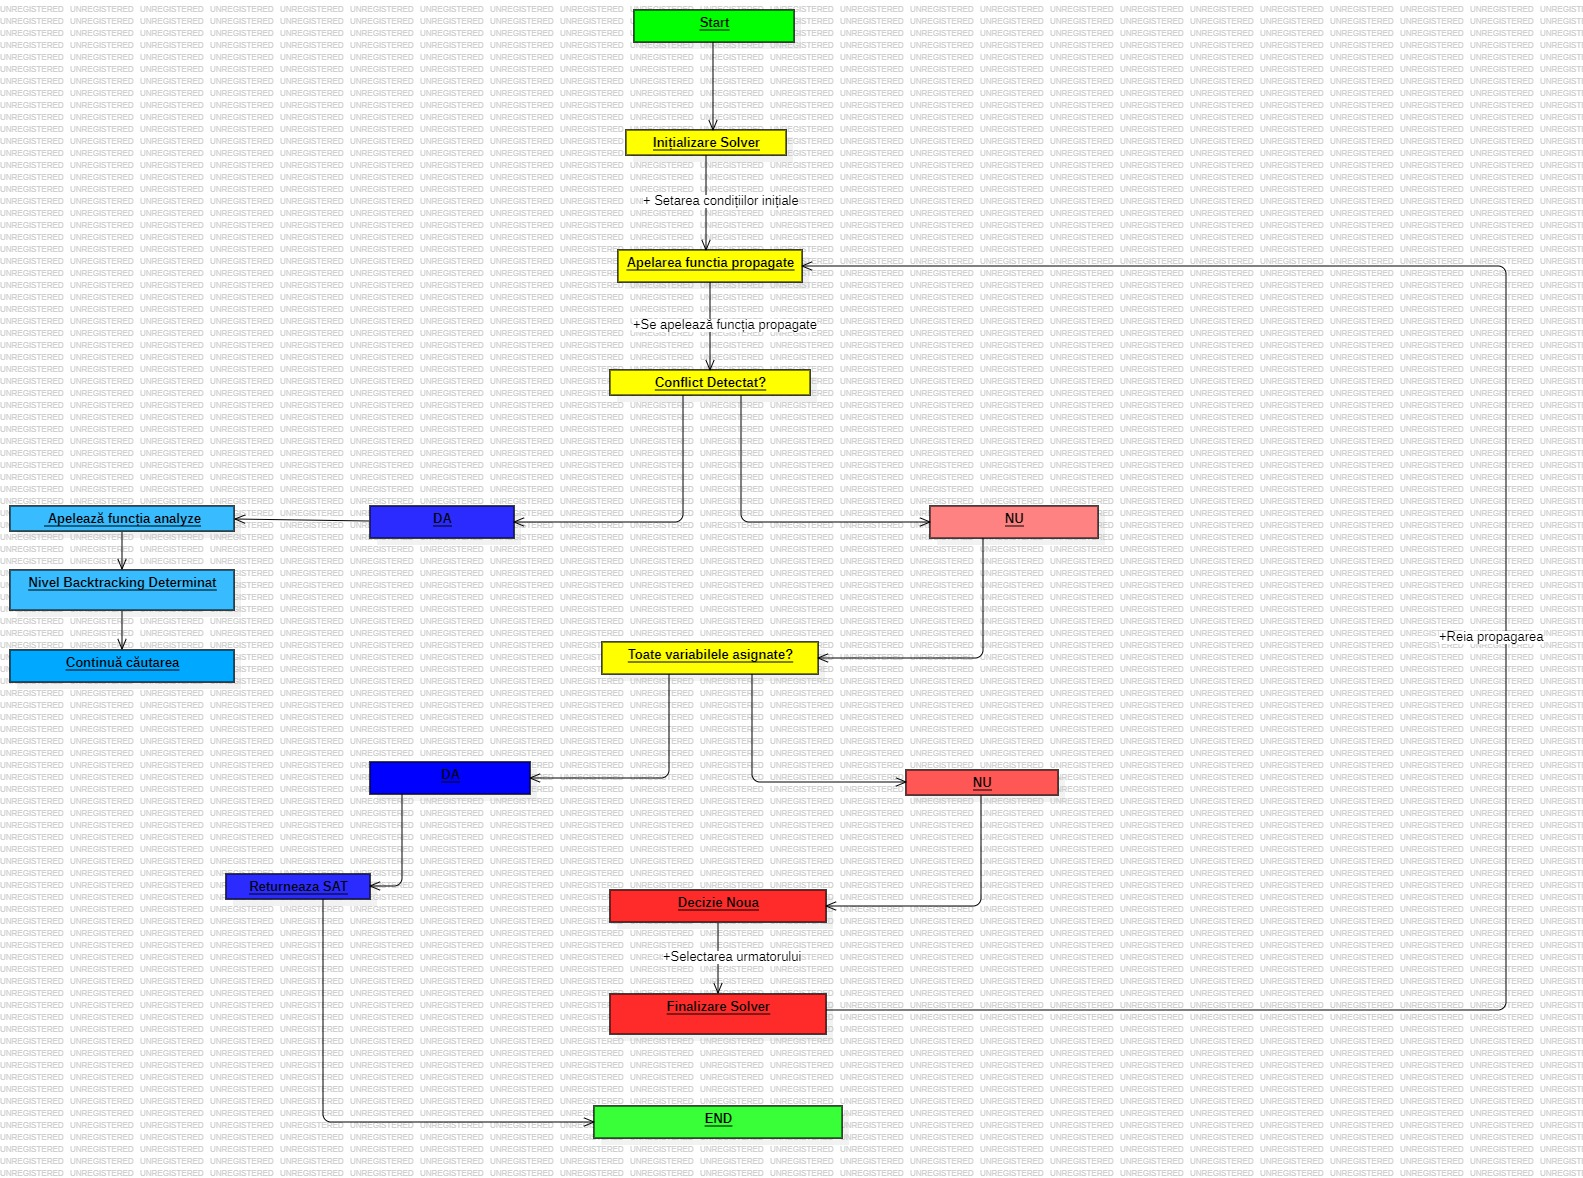
\includegraphics[height=8cm]{Model2!solver_3.jpg} 
    \label{fig:sample}
\end{figure}
\newpage
\textbf{*propagate function}
\\
Both the DPLL (Davis-Putnam-Logemann-Loveland) and CDCL (Conflict-Driven Clause Learning) algorithms rely heavily on MiniSat's propagate function. Its main function is to carry out unit propagation, a crucial procedure that reduces the complexity of the SAT problem by inferring variable assignments from the solver's present state.\\
Unit propagation is an essential part of SAT solving that takes advantage of the fact that if a clause has all but one of its literals assigned a value, the value of the remaining literal is automatically determined. This is so because only when at least one of a clause's literals is true can it be said to be satisfied. The unassigned literal must be assigned in a manner that fulfills the condition if there is only one unassigned literal and the clause is not satisfied. This deduction speeds up the solving process and narrows the search space.
\\
Steps of the propagation function:
\begin{itemize}
\item MiniSat uses the two-literal watching technique to efficiently handle clause propagation. In this method, instead of keeping track of all literals in a clause, the solver only watches two literals at a time. 
\item Each clause in the solver has two watched literals, which are chosen in a way that allows efficient detection of when a clause is unit (i.e., has only one unassigned literal). When a literal is assigned, the solver checks the watched literals and updates the clause accordingly.
Triggering Propagation:

\item The propagate function starts by examining all clauses with unassigned literals. If a clause has only one unassigned literal, it triggers unit propagation, forcing the assignment of the remaining literal. This is done recursively, as each new assignment might cause further assignments in other clauses.

\item During propagation, if an assignment causes a clause to become unsatisfied a conflict is detected. In that case, the solver will stop propagation and trigger conflict analysis. If a conflict is detected during propagation, the function will return a pointer to the conflicting clause, and the solver will enter the conflict resolution phase (via the analyze function).

\item MiniSat's use of two-literal watching ensures that propagation is done efficiently. Only the minimal necessary checks are made, and updates to the clause database are handled quickly.
By monitoring the status of every literal in the current decision level, the function also makes sure the solver doesn't do unnecessary checks.
\end{itemize}

 \begin{figure}[h] 
    \centering
    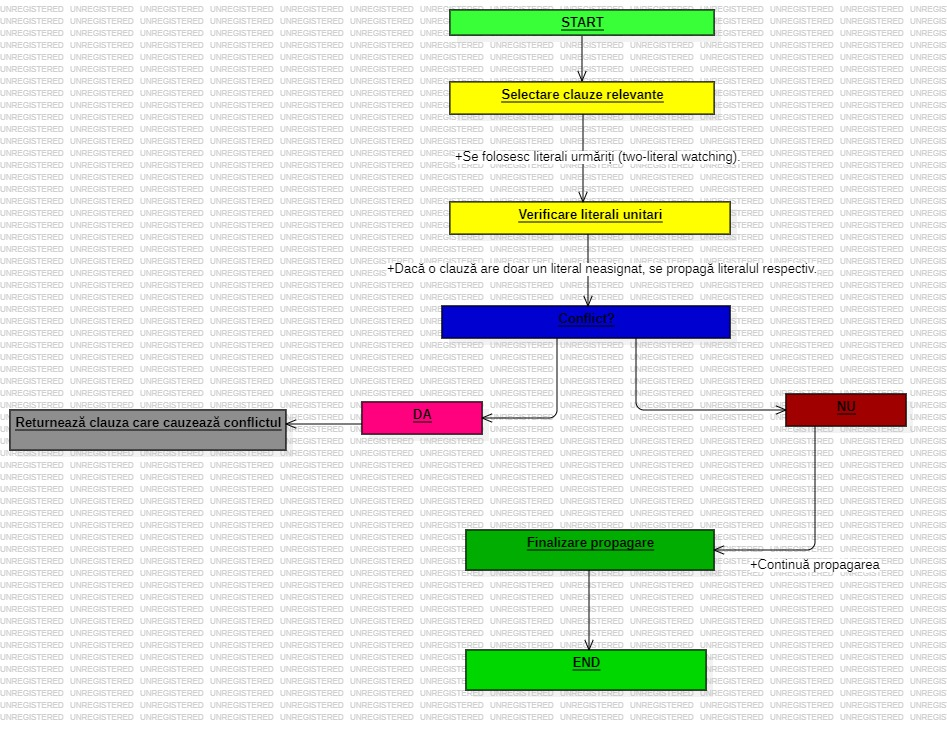
\includegraphics[height=8cm]{Propagate.jpg} 
    \label{fig:sample}
\end{figure}


\textbf{*analyze function}
\\
When a conflict is detected during unit propagation, analyze is responsible for diagnosing the conflict, deriving a learned clause, and determining the appropriate backtracking level. This allows the solver to avoid redundant searches and focus on more promising parts of the search space. 
\\
Steps if the analyze function:
\begin{itemize}
    \item When a conflict is detected during propagation, the analyze function is invoked with the conflicting clause as input. Finding the conflicting literals that led to the conflict is the first stage of analysis. 

\item The analyze function traces the conflict backward using a technique called First-UIP (Unique Implication Point). The idea is to identify the point at which the conflict could have been avoided by making a different decision.
First-UIP analysis traces the conflicting literals backward, determining the implication chain. This chain is analyzed to derive the learned clause, which will help prevent the solver from making the same mistake in future decision levels.

\item After tracing the conflict, the solver creates a learned clause. This clause is derived from the conflict and added to the clause database. The learned clause typically represents the condition that must hold true to avoid the conflict in the future.
The learned clause is typically a non-chronological clause, meaning it involves literals from multiple decision levels. This allows the solver to avoid the specific conflict by skipping over the erroneous search path.


\item A critical aspect of CDCL solvers like MiniSat is non-chronological backtracking. After deriving a learned clause, the solver must determine the appropriate backtrack level. This level is not necessarily the most recent decision level but the one that allows the solver to skip over the conflict and explore different paths. 

\item The learned clause is utilized in later propagations to avoid the same conflict after it has been derived and put to the clause database. 

\item To ensure the learned clause is as small and concise as possible, MiniSat applies clause minimization techniques. This step attempts to remove any unnecessary literals from the learned clause, making it more efficient in future propagation.
\end{itemize}
 \begin{figure}[h] 
    \centering
    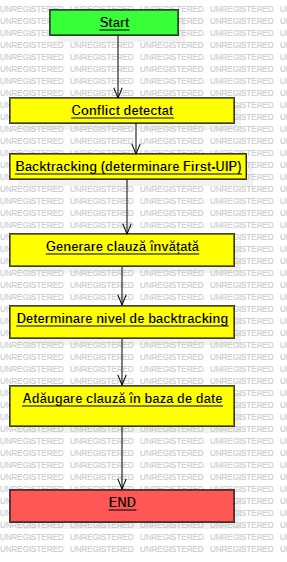
\includegraphics[height=8cm]{Model3!analyze_4.jpg} 
    \label{fig:sample}
\end{figure}
\newpage
\textbf{*simplify function}
\\
 It is typically used to remove clauses or literals that are redundant or unnecessary, which helps in improving both the performance and memory usage of the solver. This function is particularly important in the context of the Conflict-Driven Clause Learning (CDCL) algorithm, where learned clauses accumulate over time, potentially leading to a larger clause database that could degrade performance.\cite{minisatgit}
 \\
 The key operations in simplification include:
 \begin{itemize}
     \item Eliminate redundant clauses.
    \item Remove literals that are no longer needed.
    \item Reduce the size of learned clauses for better performance.
    \item Perform simplification dynamically during the solving process to keep the clause database relevant.
 \end{itemize}
  \begin{figure}[h] 
    \centering
    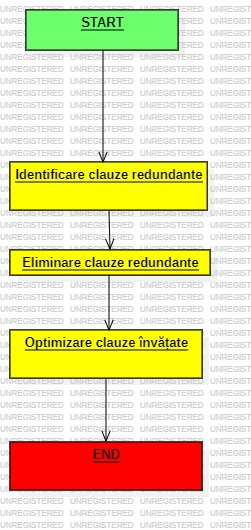
\includegraphics[height=8cm]{Model4!simplify_5.jpg} 
    \label{fig:sample}
\end{figure}
\newpage
 \subsection{Use of MiniSat in debug mode}
MinisatSat was used in debug mode on WSL Ubuntu and using gdb command(GNU Debugger). For this part it was created a smaller benchmark with very few operations so that the steps the tool makes could be more visible and also to reduce the processing time. The file created contains 6 variables and 11 clauses.
Multiple breakpoints were placed in several function e.g. main function, analyze, propagate and pickBranchLit. During this debugging session the workflow of MiniSat was observed. First the tool correctly parsed the CNF file with 6 variables and 11 clauses, the problem's clauses were loaded into the solver's internal data structure without errors. Then for the simplification the eliminate function was called, but due to the fact that the problem was very simple no clauses were removed. Afterwards, the solver repeatedly invoked propagate function to deduce variable assignments from unit clauses, a total of 6 propagations took place, which indicated that the solver was able to simplify the problem significantly. It was observed that the function pickBranchLit was invoked once, meaning MiniSat made a single decision on which variable to assign to a value. This led to further propagation, which resolved all remaining clauses without encountering conflicts. No conflicts occurred, so analyze function was never triggered, which means that the problem was simple enough to be solved without backtracking and clause learning. MiniSat performed one restart, but since no conflicts were present, the restart had no substantial effect. In the end, the solver determined the problem to be SATISFIABLE.
\\
\textbf{Observation of DPLL and CDCL}
\\
The DPLL reduced the problem by propagating logical implications from unit clauses. The solver made one heuristic-based decision, which was sufficient to deduce all other variable assignments through propagation. Typically DPLL involves backtracking when conflicts are encountered, but since no problem was encountered in this case, backtracking was not necessary. CDCL builds on DPLL by adding the ability to learn from conflicts, when these occur new clauses are added to the database to prevent the solver from explrong the same incorrect assignemnt. Since, no conflict was present, this part was not used. CDCL uses restarts to escape possible dead-ends, the tool performed one restart but had no significant impact due to lack of conflicts. 
\\
\textbf{Implementation of UIP view}
\\
In the context of SAT solvers such as MiniSati, Unique Implication Point is the first literal found in a conflict graph traversal that belongs to the current decision level. The 'analyze' function processes the conflict clause and the literals are traversed backward through their reason clauses. The counter 'pathC' keeps track of the unresolved literals at the current decision level. When `pathC` reaches zero, the UIP is identified, as it marks the point where all conflict dependencies converge. The negation of the UIP variable prevents revisiting the same conflict, as it becomes the asserting literal.Therefore, the conflict graph traversal continues to add literals from lower decision levels to the learnt clause while minimizing redundancy. This ensures the solver's improved performance. 
\\
Below is an example of the output when running the code with UIP detection and debugging enabled:
\begin{verbatim}
Starting conflict analysis...
Conflict clause literals: 5 6 7
Literal 5 is at the current decision level.
Literal 6 is at the current decision level.
Literal 7 is added to the learnt clause.
Traversing reason clause for literal 6: 3 4
Literal 4 is added to the learnt clause.
Traversing reason clause for literal 5: 1 2
Found UIP: 6 at decision level 3
Learnt clause including UIP: 6 7 4 2
\end{verbatim}

\section{Conclusions}

   The presented experiment showed that CNF files with a more complex structure, that contain a larger number of variables and clauses, have significantly higher execution times. This is consistent with theory, since in general, more complex problems require more propagations and conflicts to solve. The MiniSAT solver efficiently handles problems of different levels of complexity, using tools designed for optimization, such as CDCL and DPLL algorithms, heuristics. These tools help reduce the search space and increase performance in general. The differences between the two computers used in the experiment revealed that although processor frequency and operating system can influence performance, they are not always decisive for execution times.  The theoretical notions studied in the course, such as DPLL, CDCL algorithms and heuristics for variable selection, were successfully applied in the analysis of the CNF files components of the random-circuit benchmark. This provided a deeper understanding of how SAT algorithms operate in real-world scenarios. The distribution of variables and clauses in SAT problems also has a major impact on algorithm performance. Well-structured problems and those with fewer internal conflicts were solved in a shorter time.



\begin{credits}
\subsubsection{\ackname} Ioana Todoca was responsible for running the benchmarks in MiniSAT, for creating the bash script that was used for automatisation and efficiency, for running the code in the debug mode, modifyng the MiniSat code(implementation of UIP view) and also for the writing of the documentation. Iulia Modoaca was responsible for running the benchmarks, doing the comparison between the two computers used for the experiment and for writing the documentation as well. Miruna Sapca and Bogdan Jude did part of the research and contributed in writing the documentation and final presentation.

\end{credits}
%
% ---- Bibliography ----
%
% BibTeX users should specify bibliography style 'splncs04'.
% References will then be sorted and formatted in the correct style.
%
% \bibliographystyle{splncs04}
% \bibliography{mybibliography}
%
\begin{thebibliography}{8}
\bibitem[1]
\\Fadi Aloul et al. - “Solving Difficult Instances of Boolean Satisfiability in the Presence of Symmetry,” IEEE Transactions on Computer-Aided Design, 22(9), pp. 1117-1137, 20031
\bibitem[2]
\\SATLIB - Benchmark Problems - This resource provides a collection of satisfiable and unsatisfiable SAT benchmark instances.

\bibitem[3]
\\Mitiq Documentation - “Benchmarking Circuits,” which includes information on random gate sequences for evaluating error rates.

\bibitem[4]
\\Balyo, T., Gableske, O.,  Sinz, C. (2004). Restoring circuit structure from SAT instances. International Workshop on Logic Synthesis (IWLS). 

\bibitem[5]
\\Ke Xu et al. - “SAT Benchmarks for Randomized Urquhart Problems,” which provides a collection of CNF problems for SAT solvers


\end{thebibliography}
\end{document}
